\chapter{Конструкторская часть}

В аналитической части работы была представлена концептуальная модель процесса извлечения информации, визуализированная с помощью IDEF0 диаграммы. 
На основе этого анализа в конструкторской части рассматриваются детали процессов, происходящих внутри, которые и выявляют необъходимые сущности с использованием больших языковых моделей (LLM).

\section{Детали алгоритма}

\begin{figure}[H]
    \centering
    \includegraphics[width=1\textwidth]{C:/MGTU/ai\_kursach/report/images/ramus/02\_A0.png}
    \caption{Алгоритм определения акторов, действий и временных характеристик}
    \label{fig:idef0_1}
\end{figure}

Диаграмма (рис. \ref{fig:idef0_1}) представляет IDEF0-модель процесса извлечения сущностей, в которой опускается этап взаимодействия с пользователем.

\subsection{Алгоритмы обработки}

\subsubsection{Предобработка}
Перед анализом текста производится его предварительная обработка, которая включает в себя:
\begin{itemize}
    \item удаление лишних пробельных символов, переносов строк и иных символов;
    \item очистка от неинформативных элементов, таких как специальные символы, HTML-теги и т.д;
    \item разделение текста на логические фрагменты (абзацы, предложения).
\end{itemize}

\subsubsection{Формирование промпта}
Для корректной работы LLM необходимо сформировать промпт, содержащий четкую инструкцию для модели. 
В случае Instruct-версий моделей применяется формат явных директив. 

Например, текст может быть представлен в следующем виде:
\begin{verbatim}
[INST] Определи акторов, их действия и временные характеристики. 
Представь результат в формате JSON. [/INST]
Текст: "В 2023 году исследователь написал статью."
\end{verbatim}

Такой подход уменьшает вероятности появления ошибок в неправильной интерпретации промпта, что улучшает качество ответа.

\subsubsection{Выявление сущностей}
На этом этапе происходит автоматическое определение акторов, их действий и временных характеристик на основе обученных представлений модели, 
повлиять на который можно только через конфигурационный файл модели.

\subsubsection{Постобработка}

После получения ответа от модели выполняется его дополнительная обработка:
\begin{itemize}
    \item проверяется соответствие выходного формата запрашиваемому (например, если ответ должен быть в формате JSON, производится валидация структуры);
    \item выделяются только те элементы, которые требовалось определить, устраняя возможные избыточные данные.
\end{itemize}

\section{Взаимодействие с системой}

\begin{figure}[H]
    \centering
    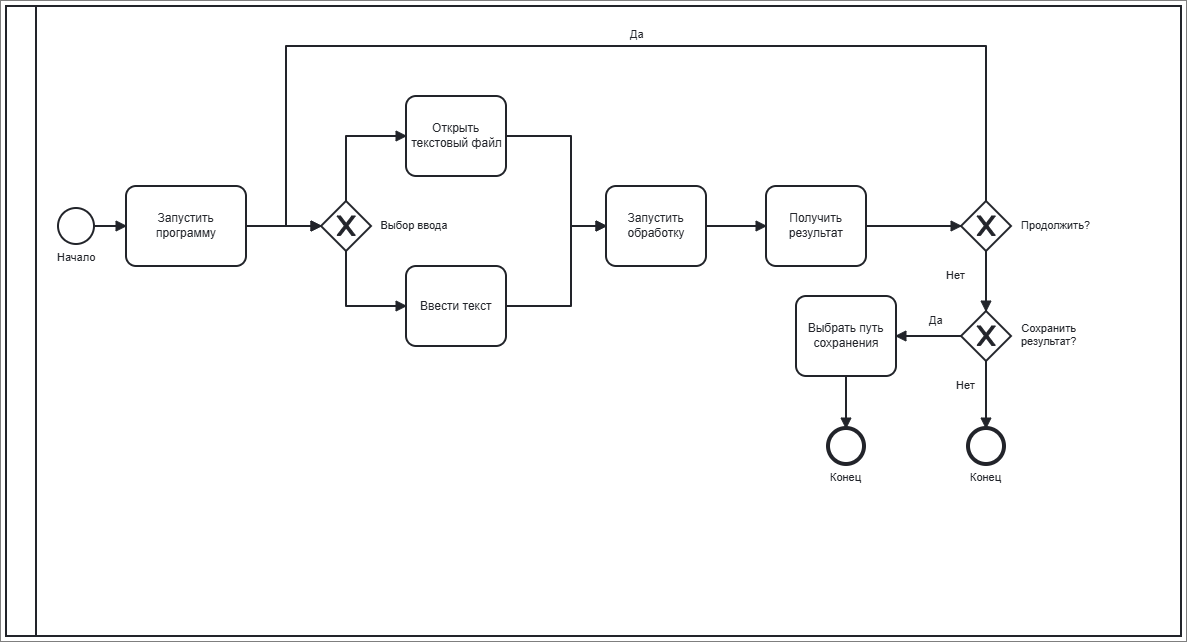
\includegraphics[width=1\textwidth]{C:/MGTU/ai\_kursach/report/images/Algos.png}
    \caption{Алгоритм взимодейсвия с системой}
    \label{fig:userToSystem}
\end{figure}

На рисунке \ref{fig:userToSystem} представлен алгоритм взаимодействие пользователя с системой посредством консольного либо графического приложения. 
В обоих случаях, исходный текст для анализа вводится пользователем либо непосредственно в поле ввода интерфейса, либо загружается из текстового файла. 
Обработка текста инициируется пользователем. Результаты анализа представляются различными способами в зависимости от типа интерфейса. 
В графическом приложении производится визуализация: извлеченные сущности (акторы, действия, временные характеристики) 
выделяются различными цветами непосредственно в тексте (например, акторы – красным цветом, действия – зеленым, временные характеристики – оранжевым). 
В консольном приложении вывод результатов осуществляется в текстовом формате, с явным указанием принадлежности каждого элемента к определенной категории сущностей. 
Дополнительно, вне зависимости от типа интерфейса, предусмотрена возможность сохранения результатов анализа в файл формата JSON для последующей обработки или интеграции 
с другими системами.

\subsection{Конфигурационный файл}

Для тонкой настройки процесса обработки текста и представления результатов используется конфигурационный файл в формате JSON.  
Данный файл позволяет пользователю задать ряд параметров, влияющих на поведение системы, такие как:
\begin{itemize}
    \item шаблон промпта;
    \item формат вывода;
    \item цветовая схема (для графического интерфейса);
    \item путь к файлу с текстом по умолчанию;
    \item температура модели (отвечает за случайность сгенерированного текста);
\end{itemize}

\section*{Вывод}

Разработанная архитектура демонстрирует модульный и масштабируемый подход к автоматизированному извлечению акторов, действий и временных характеристик из текстовых данных с использованием больших языковых моделей. 
Детально описаны этапы: предобработка текста, формирование четкого запроса к модели, автоматическое выявление сущностей и последующая постобработка.
Предусмотрены возможные варианты взаимодействия с системой — графический интерфейс с визуальной подсветкой ключевых элементов 
и консольное приложение для текстового вывода. 
Гибкая настройка параметров через конфигурационный файл в формате JSON позволяет адаптировать систему под различные условия эксплуатации.


\clearpage